\documentclass[1p]{elsarticle_modified}
%\bibliographystyle{elsarticle-num}

%\usepackage[colorlinks]{hyperref}
%\usepackage{abbrmath_seonhwa} %\Abb, \Ascr, \Acal ,\Abf, \Afrak
\usepackage{amsfonts}
\usepackage{amssymb}
\usepackage{amsmath}
\usepackage{amsthm}
\usepackage{scalefnt}
\usepackage{amsbsy}
\usepackage{kotex}
\usepackage{caption}
\usepackage{subfig}
\usepackage{color}
\usepackage{graphicx}
\usepackage{xcolor} %% white, black, red, green, blue, cyan, magenta, yellow
\usepackage{float}
\usepackage{setspace}
\usepackage{hyperref}

\usepackage{tikz}
\usetikzlibrary{arrows}

\usepackage{multirow}
\usepackage{array} % fixed length table
\usepackage{hhline}

%%%%%%%%%%%%%%%%%%%%%
\makeatletter
\renewcommand*\env@matrix[1][\arraystretch]{%
	\edef\arraystretch{#1}%
	\hskip -\arraycolsep
	\let\@ifnextchar\new@ifnextchar
	\array{*\c@MaxMatrixCols c}}
\makeatother %https://tex.stackexchange.com/questions/14071/how-can-i-increase-the-line-spacing-in-a-matrix
%%%%%%%%%%%%%%%

\usepackage[normalem]{ulem}

\newcommand{\msout}[1]{\ifmmode\text{\sout{\ensuremath{#1}}}\else\sout{#1}\fi}
%SOURCE: \msout is \stkout macro in https://tex.stackexchange.com/questions/20609/strikeout-in-math-mode

\newcommand{\cancel}[1]{
	\ifmmode
	{\color{red}\msout{#1}}
	\else
	{\color{red}\sout{#1}}
	\fi
}

\newcommand{\add}[1]{
	{\color{blue}\uwave{#1}}
}

\newcommand{\replace}[2]{
	\ifmmode
	{\color{red}\msout{#1}}{\color{blue}\uwave{#2}}
	\else
	{\color{red}\sout{#1}}{\color{blue}\uwave{#2}}
	\fi
}

\newcommand{\Sol}{\mathcal{S}} %segment
\newcommand{\D}{D} %diagram
\newcommand{\A}{\mathcal{A}} %arc


%%%%%%%%%%%%%%%%%%%%%%%%%%%%%5 test

\def\sl{\operatorname{\textup{SL}}(2,\Cbb)}
\def\psl{\operatorname{\textup{PSL}}(2,\Cbb)}
\def\quan{\mkern 1mu \triangleright \mkern 1mu}

\theoremstyle{definition}
\newtheorem{thm}{Theorem}[section]
\newtheorem{prop}[thm]{Proposition}
\newtheorem{lem}[thm]{Lemma}
\newtheorem{ques}[thm]{Question}
\newtheorem{cor}[thm]{Corollary}
\newtheorem{defn}[thm]{Definition}
\newtheorem{exam}[thm]{Example}
\newtheorem{rmk}[thm]{Remark}
\newtheorem{alg}[thm]{Algorithm}

\newcommand{\I}{\sqrt{-1}}
\begin{document}

%\begin{frontmatter}
%
%\title{Boundary parabolic representations of knots up to 8 crossings}
%
%%% Group authors per affiliation:
%\author{Yunhi Cho} 
%\address{Department of Mathematics, University of Seoul, Seoul, Korea}
%\ead{yhcho@uos.ac.kr}
%
%
%\author{Seonhwa Kim} %\fnref{s_kim}}
%\address{Center for Geometry and Physics, Institute for Basic Science, Pohang, 37673, Korea}
%\ead{ryeona17@ibs.re.kr}
%
%\author{Hyuk Kim}
%\address{Department of Mathematical Sciences, Seoul National University, Seoul 08826, Korea}
%\ead{hyukkim@snu.ac.kr}
%
%\author{Seokbeom Yoon}
%\address{Department of Mathematical Sciences, Seoul National University, Seoul, 08826,  Korea}
%\ead{sbyoon15@snu.ac.kr}
%
%\begin{abstract}
%We find all boundary parabolic representation of knots up to 8 crossings.
%
%\end{abstract}
%\begin{keyword}
%    \MSC[2010] 57M25 
%\end{keyword}
%
%\end{frontmatter}

%\linenumbers
%\tableofcontents
%
\newcommand\colored[1]{\textcolor{white}{\rule[-0.35ex]{0.8em}{1.4ex}}\kern-0.8em\color{red} #1}%
%\newcommand\colored[1]{\textcolor{white}{ #1}\kern-2.17ex	\textcolor{white}{ #1}\kern-1.81ex	\textcolor{white}{ #1}\kern-2.15ex\color{red}#1	}

{\Large $\underline{12a_{0059}~(K12a_{0059})}$}

\setlength{\tabcolsep}{10pt}
\renewcommand{\arraystretch}{1.6}
\vspace{1cm}\begin{tabular}{m{100pt}>{\centering\arraybackslash}m{274pt}}
\multirow{5}{120pt}{
	\centering
	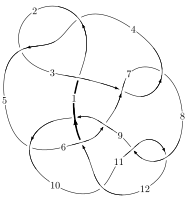
\includegraphics[width=112pt]{../../../GIT/diagram.site/Diagrams/png/860_12a_0059.png}\\
\ \ \ A knot diagram\footnotemark}&
\allowdisplaybreaks
\textbf{Linearized knot diagam} \\
\cline{2-2}
 &
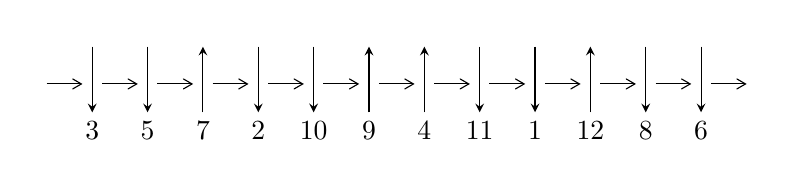
\begin{tikzpicture}[x=20pt, y=17pt]
	% nodes
	\node (C0) at (0, 0) {};
	\node (C1) at (1, 0) {};
	\node (C1U) at (1, +1) {};
	\node (C1D) at (1, -1) {3};

	\node (C2) at (2, 0) {};
	\node (C2U) at (2, +1) {};
	\node (C2D) at (2, -1) {5};

	\node (C3) at (3, 0) {};
	\node (C3U) at (3, +1) {};
	\node (C3D) at (3, -1) {7};

	\node (C4) at (4, 0) {};
	\node (C4U) at (4, +1) {};
	\node (C4D) at (4, -1) {2};

	\node (C5) at (5, 0) {};
	\node (C5U) at (5, +1) {};
	\node (C5D) at (5, -1) {10};

	\node (C6) at (6, 0) {};
	\node (C6U) at (6, +1) {};
	\node (C6D) at (6, -1) {9};

	\node (C7) at (7, 0) {};
	\node (C7U) at (7, +1) {};
	\node (C7D) at (7, -1) {4};

	\node (C8) at (8, 0) {};
	\node (C8U) at (8, +1) {};
	\node (C8D) at (8, -1) {11};

	\node (C9) at (9, 0) {};
	\node (C9U) at (9, +1) {};
	\node (C9D) at (9, -1) {1};

	\node (C10) at (10, 0) {};
	\node (C10U) at (10, +1) {};
	\node (C10D) at (10, -1) {12};

	\node (C11) at (11, 0) {};
	\node (C11U) at (11, +1) {};
	\node (C11D) at (11, -1) {8};

	\node (C12) at (12, 0) {};
	\node (C12U) at (12, +1) {};
	\node (C12D) at (12, -1) {6};
	\node (C13) at (13, 0) {};

	% arrows
	\draw[->,>={angle 60}]
	(C0) edge (C1) (C1) edge (C2) (C2) edge (C3) (C3) edge (C4) (C4) edge (C5) (C5) edge (C6) (C6) edge (C7) (C7) edge (C8) (C8) edge (C9) (C9) edge (C10) (C10) edge (C11) (C11) edge (C12) (C12) edge (C13) ;	\draw[->,>=stealth]
	(C1U) edge (C1D) (C2U) edge (C2D) (C3D) edge (C3U) (C4U) edge (C4D) (C5U) edge (C5D) (C6D) edge (C6U) (C7D) edge (C7U) (C8U) edge (C8D) (C9U) edge (C9D) (C10D) edge (C10U) (C11U) edge (C11D) (C12U) edge (C12D) ;
	\end{tikzpicture} \\
\hhline{~~} \\& 
\textbf{Solving Sequence} \\ \cline{2-2} 
 &
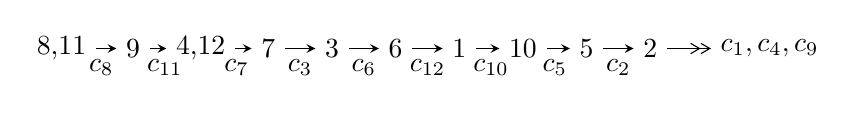
\begin{tikzpicture}[x=23pt, y=7pt]
	% node
	\node (A0) at (-1/8, 0) {8,11};
	\node (A1) at (1, 0) {9};
	\node (A2) at (33/16, 0) {4,12};
	\node (A3) at (25/8, 0) {7};
	\node (A4) at (33/8, 0) {3};
	\node (A5) at (41/8, 0) {6};
	\node (A6) at (49/8, 0) {1};
	\node (A7) at (57/8, 0) {10};
	\node (A8) at (65/8, 0) {5};
	\node (A9) at (73/8, 0) {2};
	\node (C1) at (1/2, -1) {$c_{8}$};
	\node (C2) at (3/2, -1) {$c_{11}$};
	\node (C3) at (21/8, -1) {$c_{7}$};
	\node (C4) at (29/8, -1) {$c_{3}$};
	\node (C5) at (37/8, -1) {$c_{6}$};
	\node (C6) at (45/8, -1) {$c_{12}$};
	\node (C7) at (53/8, -1) {$c_{10}$};
	\node (C8) at (61/8, -1) {$c_{5}$};
	\node (C9) at (69/8, -1) {$c_{2}$};
	\node (A10) at (11, 0) {$c_{1},c_{4},c_{9}$};

	% edge
	\draw[->,>=stealth]	
	(A0) edge (A1) (A1) edge (A2) (A2) edge (A3) (A3) edge (A4) (A4) edge (A5) (A5) edge (A6) (A6) edge (A7) (A7) edge (A8) (A8) edge (A9) ;
	\draw[->>,>={angle 60}]	
	(A9) edge (A10);
\end{tikzpicture} \\ 

\end{tabular} \\

\footnotetext{
The image of knot diagram is generated by the software ``\textbf{Draw programme}" developed by Andrew Bartholomew(\url{http://www.layer8.co.uk/maths/draw/index.htm\#Running-draw}), where we modified some parts for our purpose(\url{https://github.com/CATsTAILs/LinksPainter}).
}\phantom \\ \newline 
\centering \textbf{Ideals for irreducible components\footnotemark of $X_{\text{par}}$} 
 
\begin{align*}
I^u_{1}&=\langle 
-4.71088\times10^{361} u^{137}-4.89757\times10^{362} u^{136}+\cdots+2.81012\times10^{363} b+2.16214\times10^{363},\\
\phantom{I^u_{1}}&\phantom{= \langle  }3.37731\times10^{362} u^{137}-1.72512\times10^{363} u^{136}+\cdots+2.81012\times10^{363} a+1.76728\times10^{364},\\
\phantom{I^u_{1}}&\phantom{= \langle  }u^{138}+2 u^{137}+\cdots-14 u+1\rangle \\
I^u_{2}&=\langle 
b,\;u^8+2 u^7+3 u^6+2 u^5+3 u^4+2 u^3+2 u^2+a+1,\;u^9+u^8+2 u^7+u^6+3 u^5+u^4+2 u^3+u-1\rangle \\
\\
\end{align*}
\raggedright * 2 irreducible components of $\dim_{\mathbb{C}}=0$, with total 147 representations.\\
\footnotetext{All coefficients of polynomials are rational numbers. But the coefficients are sometimes approximated in decimal forms when there is not enough margin.}
\newpage
\renewcommand{\arraystretch}{1}
\centering \section*{I. $I^u_{1}= \langle -4.71\times10^{361} u^{137}-4.90\times10^{362} u^{136}+\cdots+2.81\times10^{363} b+2.16\times10^{363},\;3.38\times10^{362} u^{137}-1.73\times10^{363} u^{136}+\cdots+2.81\times10^{363} a+1.77\times10^{364},\;u^{138}+2 u^{137}+\cdots-14 u+1 \rangle$}
\flushleft \textbf{(i) Arc colorings}\\
\begin{tabular}{m{7pt} m{180pt} m{7pt} m{180pt} }
\flushright $a_{8}=$&$\begin{pmatrix}1\\0\end{pmatrix}$ \\
\flushright $a_{11}=$&$\begin{pmatrix}0\\u\end{pmatrix}$ \\
\flushright $a_{9}=$&$\begin{pmatrix}1\\u^2\end{pmatrix}$ \\
\flushright $a_{4}=$&$\begin{pmatrix}-0.120184 u^{137}+0.613895 u^{136}+\cdots+15.1732 u-6.28898\\0.0167640 u^{137}+0.174283 u^{136}+\cdots+12.4843 u-0.769412\end{pmatrix}$ \\
\flushright $a_{12}=$&$\begin{pmatrix}- u\\u\end{pmatrix}$ \\
\flushright $a_{7}=$&$\begin{pmatrix}-0.560792 u^{137}-0.490800 u^{136}+\cdots-47.6605 u+3.40798\\0.180158 u^{137}+0.477905 u^{136}+\cdots+9.60968 u-1.21932\end{pmatrix}$ \\
\flushright $a_{3}=$&$\begin{pmatrix}0.618598 u^{137}+1.87938 u^{136}+\cdots+60.5458 u-12.1743\\-0.0179355 u^{137}+0.0130907 u^{136}+\cdots+5.49317 u+0.408548\end{pmatrix}$ \\
\flushright $a_{6}=$&$\begin{pmatrix}-0.849545 u^{137}-1.94068 u^{136}+\cdots-47.8784 u+3.99652\\0.333855 u^{137}+0.868326 u^{136}+\cdots-2.31475 u-0.346952\end{pmatrix}$ \\
\flushright $a_{1}=$&$\begin{pmatrix}-0.287569 u^{137}+0.783730 u^{136}+\cdots-31.9924 u+4.35349\\-1.43846 u^{137}-2.79732 u^{136}+\cdots+21.5369 u-1.72603\end{pmatrix}$ \\
\flushright $a_{10}=$&$\begin{pmatrix}- u^3\\u^3+u\end{pmatrix}$ \\
\flushright $a_{5}=$&$\begin{pmatrix}-0.767107 u^{137}-1.00356 u^{136}+\cdots-57.8502 u+4.70515\\0.200522 u^{137}+0.538058 u^{136}+\cdots+10.8465 u-1.34799\end{pmatrix}$ \\
\flushright $a_{2}=$&$\begin{pmatrix}-0.458501 u^{137}+0.239804 u^{136}+\cdots-11.9475 u-5.01052\\0.119330 u^{137}+0.460278 u^{136}+\cdots+19.9372 u-1.43411\end{pmatrix}$\\&\end{tabular}
\flushleft \textbf{(ii) Obstruction class $= -1$}\\~\\
\flushleft \textbf{(iii) Cusp Shapes $= -3.92502 u^{137}-8.32211 u^{136}+\cdots-15.6428 u-3.22352$}\\~\\
\newpage\renewcommand{\arraystretch}{1}
\flushleft \textbf{(iv) u-Polynomials at the component}\newline \\
\begin{tabular}{m{50pt}|m{274pt}}
Crossings & \hspace{64pt}u-Polynomials at each crossing \\
\hline $$\begin{aligned}c_{1}\end{aligned}$$&$\begin{aligned}
&u^{138}+70 u^{137}+\cdots-82 u+1
\end{aligned}$\\
\hline $$\begin{aligned}c_{2},c_{4}\end{aligned}$$&$\begin{aligned}
&u^{138}-10 u^{137}+\cdots+14 u-1
\end{aligned}$\\
\hline $$\begin{aligned}c_{3},c_{7}\end{aligned}$$&$\begin{aligned}
&u^{138}- u^{137}+\cdots+4096 u+512
\end{aligned}$\\
\hline $$\begin{aligned}c_{5}\end{aligned}$$&$\begin{aligned}
&u^{138}+2 u^{137}+\cdots-2626 u-97
\end{aligned}$\\
\hline $$\begin{aligned}c_{6}\end{aligned}$$&$\begin{aligned}
&u^{138}+6 u^{137}+\cdots-67104 u-2117
\end{aligned}$\\
\hline $$\begin{aligned}c_{8},c_{11}\end{aligned}$$&$\begin{aligned}
&u^{138}-2 u^{137}+\cdots+14 u+1
\end{aligned}$\\
\hline $$\begin{aligned}c_{9}\end{aligned}$$&$\begin{aligned}
&u^{138}-14 u^{137}+\cdots-2 u+1
\end{aligned}$\\
\hline $$\begin{aligned}c_{10}\end{aligned}$$&$\begin{aligned}
&u^{138}-54 u^{137}+\cdots+14 u+1
\end{aligned}$\\
\hline $$\begin{aligned}c_{12}\end{aligned}$$&$\begin{aligned}
&u^{138}-10 u^{137}+\cdots+2 u-1
\end{aligned}$\\
\hline
\end{tabular}\\~\\
\newpage\renewcommand{\arraystretch}{1}
\flushleft \textbf{(v) Riley Polynomials at the component}\newline \\
\begin{tabular}{m{50pt}|m{274pt}}
Crossings & \hspace{64pt}Riley Polynomials at each crossing \\
\hline $$\begin{aligned}c_{1}\end{aligned}$$&$\begin{aligned}
&y^{138}+6 y^{137}+\cdots-5018 y+1
\end{aligned}$\\
\hline $$\begin{aligned}c_{2},c_{4}\end{aligned}$$&$\begin{aligned}
&y^{138}-70 y^{137}+\cdots+82 y+1
\end{aligned}$\\
\hline $$\begin{aligned}c_{3},c_{7}\end{aligned}$$&$\begin{aligned}
&y^{138}-57 y^{137}+\cdots-8912896 y+262144
\end{aligned}$\\
\hline $$\begin{aligned}c_{5}\end{aligned}$$&$\begin{aligned}
&y^{138}-166 y^{137}+\cdots+9748742 y+9409
\end{aligned}$\\
\hline $$\begin{aligned}c_{6}\end{aligned}$$&$\begin{aligned}
&y^{138}-118 y^{137}+\cdots-1356064422 y+4481689
\end{aligned}$\\
\hline $$\begin{aligned}c_{8},c_{11}\end{aligned}$$&$\begin{aligned}
&y^{138}+54 y^{137}+\cdots-14 y+1
\end{aligned}$\\
\hline $$\begin{aligned}c_{9}\end{aligned}$$&$\begin{aligned}
&y^{138}-10 y^{137}+\cdots-14 y+1
\end{aligned}$\\
\hline $$\begin{aligned}c_{10}\end{aligned}$$&$\begin{aligned}
&y^{138}+62 y^{137}+\cdots+2378 y+1
\end{aligned}$\\
\hline $$\begin{aligned}c_{12}\end{aligned}$$&$\begin{aligned}
&y^{138}-14 y^{137}+\cdots-10 y+1
\end{aligned}$\\
\hline
\end{tabular}\\~\\
\newpage\flushleft \textbf{(vi) Complex Volumes and Cusp Shapes}
$$\begin{array}{c|c|c}  
\text{Solutions to }I^u_{1}& \I (\text{vol} + \sqrt{-1}CS) & \text{Cusp shape}\\
 \hline 
\begin{aligned}
u &= \phantom{-}0.340095 + 0.938631 I \\
a &= -2.65484 - 1.57222 I \\
b &= \phantom{-}1.084210 + 0.480895 I\end{aligned}
 & \phantom{-}0.93099 + 3.37995 I & \phantom{-0.000000 } 0 \\ \hline\begin{aligned}
u &= \phantom{-}0.340095 - 0.938631 I \\
a &= -2.65484 + 1.57222 I \\
b &= \phantom{-}1.084210 - 0.480895 I\end{aligned}
 & \phantom{-}0.93099 - 3.37995 I & \phantom{-0.000000 } 0 \\ \hline\begin{aligned}
u &= -0.565847 + 0.829711 I \\
a &= -1.89250 + 1.37711 I \\
b &= \phantom{-}1.243040 + 0.380663 I\end{aligned}
 & -3.90120 + 1.41992 I & \phantom{-0.000000 } 0 \\ \hline\begin{aligned}
u &= -0.565847 - 0.829711 I \\
a &= -1.89250 - 1.37711 I \\
b &= \phantom{-}1.243040 - 0.380663 I\end{aligned}
 & -3.90120 - 1.41992 I & \phantom{-0.000000 } 0 \\ \hline\begin{aligned}
u &= \phantom{-}0.523816 + 0.842586 I \\
a &= \phantom{-}0.49491 - 4.58806 I \\
b &= \phantom{-}0.513302 - 0.642122 I\end{aligned}
 & -2.14770 - 1.10222 I & \phantom{-0.000000 } 0 \\ \hline\begin{aligned}
u &= \phantom{-}0.523816 - 0.842586 I \\
a &= \phantom{-}0.49491 + 4.58806 I \\
b &= \phantom{-}0.513302 + 0.642122 I\end{aligned}
 & -2.14770 + 1.10222 I & \phantom{-0.000000 } 0 \\ \hline\begin{aligned}
u &= \phantom{-}0.555562 + 0.842147 I \\
a &= -5.63415 + 2.08299 I \\
b &= \phantom{-}0.371240 + 0.165548 I\end{aligned}
 & -2.14622 - 2.23521 I & \phantom{-0.000000 } 0 \\ \hline\begin{aligned}
u &= \phantom{-}0.555562 - 0.842147 I \\
a &= -5.63415 - 2.08299 I \\
b &= \phantom{-}0.371240 - 0.165548 I\end{aligned}
 & -2.14622 + 2.23521 I & \phantom{-0.000000 } 0 \\ \hline\begin{aligned}
u &= \phantom{-}0.586154 + 0.792966 I \\
a &= \phantom{-}1.72146 + 0.94919 I \\
b &= \phantom{-}1.028400 + 0.569460 I\end{aligned}
 & -0.64257 + 3.65096 I & \phantom{-0.000000 } 0 \\ \hline\begin{aligned}
u &= \phantom{-}0.586154 - 0.792966 I \\
a &= \phantom{-}1.72146 - 0.94919 I \\
b &= \phantom{-}1.028400 - 0.569460 I\end{aligned}
 & -0.64257 - 3.65096 I & \phantom{-0.000000 } 0\\
 \hline 
 \end{array}$$\newpage$$\begin{array}{c|c|c}  
\text{Solutions to }I^u_{1}& \I (\text{vol} + \sqrt{-1}CS) & \text{Cusp shape}\\
 \hline 
\begin{aligned}
u &= \phantom{-}0.420026 + 0.927286 I \\
a &= \phantom{-}2.99710 + 2.14722 I \\
b &= -1.042910 - 0.202388 I\end{aligned}
 & \phantom{-}2.43266 - 1.40735 I & \phantom{-0.000000 } 0 \\ \hline\begin{aligned}
u &= \phantom{-}0.420026 - 0.927286 I \\
a &= \phantom{-}2.99710 - 2.14722 I \\
b &= -1.042910 + 0.202388 I\end{aligned}
 & \phantom{-}2.43266 + 1.40735 I & \phantom{-0.000000 } 0 \\ \hline\begin{aligned}
u &= -0.867495 + 0.535351 I \\
a &= \phantom{-}0.858232 + 0.532125 I \\
b &= -0.974643 + 0.546694 I\end{aligned}
 & -5.66343 - 4.80751 I & \phantom{-0.000000 } 0 \\ \hline\begin{aligned}
u &= -0.867495 - 0.535351 I \\
a &= \phantom{-}0.858232 - 0.532125 I \\
b &= -0.974643 - 0.546694 I\end{aligned}
 & -5.66343 + 4.80751 I & \phantom{-0.000000 } 0 \\ \hline\begin{aligned}
u &= \phantom{-}0.527672 + 0.877110 I \\
a &= \phantom{-}3.63134 + 0.70902 I \\
b &= \phantom{-}0.475349 + 0.722868 I\end{aligned}
 & -2.03184 - 3.14136 I & \phantom{-0.000000 } 0 \\ \hline\begin{aligned}
u &= \phantom{-}0.527672 - 0.877110 I \\
a &= \phantom{-}3.63134 - 0.70902 I \\
b &= \phantom{-}0.475349 - 0.722868 I\end{aligned}
 & -2.03184 + 3.14136 I & \phantom{-0.000000 } 0 \\ \hline\begin{aligned}
u &= -0.570493 + 0.859311 I \\
a &= -0.816912 + 0.512172 I \\
b &= \phantom{-}1.193220 - 0.620973 I\end{aligned}
 & -3.80516 + 3.12708 I & \phantom{-0.000000 } 0 \\ \hline\begin{aligned}
u &= -0.570493 - 0.859311 I \\
a &= -0.816912 - 0.512172 I \\
b &= \phantom{-}1.193220 + 0.620973 I\end{aligned}
 & -3.80516 - 3.12708 I & \phantom{-0.000000 } 0 \\ \hline\begin{aligned}
u &= -0.805471 + 0.534825 I \\
a &= -0.459619 + 0.647350 I \\
b &= \phantom{-}0.399102 + 0.957238 I\end{aligned}
 & -2.80156 - 2.93042 I & \phantom{-0.000000 } 0 \\ \hline\begin{aligned}
u &= -0.805471 - 0.534825 I \\
a &= -0.459619 - 0.647350 I \\
b &= \phantom{-}0.399102 - 0.957238 I\end{aligned}
 & -2.80156 + 2.93042 I & \phantom{-0.000000 } 0\\
 \hline 
 \end{array}$$\newpage$$\begin{array}{c|c|c}  
\text{Solutions to }I^u_{1}& \I (\text{vol} + \sqrt{-1}CS) & \text{Cusp shape}\\
 \hline 
\begin{aligned}
u &= -0.897882 + 0.515328 I \\
a &= \phantom{-}0.312579 - 0.760968 I \\
b &= -0.607381 - 1.045900 I\end{aligned}
 & -5.02344 - 7.63080 I & \phantom{-0.000000 } 0 \\ \hline\begin{aligned}
u &= -0.897882 - 0.515328 I \\
a &= \phantom{-}0.312579 + 0.760968 I \\
b &= -0.607381 + 1.045900 I\end{aligned}
 & -5.02344 + 7.63080 I & \phantom{-0.000000 } 0 \\ \hline\begin{aligned}
u &= -0.544617 + 0.793755 I \\
a &= -1.27517 + 0.91926 I \\
b &= \phantom{-}0.791951 + 1.123120 I\end{aligned}
 & -3.20951 - 0.12052 I & \phantom{-0.000000 } 0 \\ \hline\begin{aligned}
u &= -0.544617 - 0.793755 I \\
a &= -1.27517 - 0.91926 I \\
b &= \phantom{-}0.791951 - 1.123120 I\end{aligned}
 & -3.20951 + 0.12052 I & \phantom{-0.000000 } 0 \\ \hline\begin{aligned}
u &= \phantom{-}0.939245 + 0.442594 I \\
a &= \phantom{-}0.741341 + 0.959246 I \\
b &= -0.643323 + 0.685004 I\end{aligned}
 & -5.01384 - 0.52036 I & \phantom{-0.000000 } 0 \\ \hline\begin{aligned}
u &= \phantom{-}0.939245 - 0.442594 I \\
a &= \phantom{-}0.741341 - 0.959246 I \\
b &= -0.643323 - 0.685004 I\end{aligned}
 & -5.01384 + 0.52036 I & \phantom{-0.000000 } 0 \\ \hline\begin{aligned}
u &= \phantom{-}0.921298 + 0.258898 I \\
a &= -0.612122 + 0.342593 I \\
b &= \phantom{-}0.775567 + 0.394484 I\end{aligned}
 & -1.60499 + 0.17048 I & \phantom{-0.000000 } 0 \\ \hline\begin{aligned}
u &= \phantom{-}0.921298 - 0.258898 I \\
a &= -0.612122 - 0.342593 I \\
b &= \phantom{-}0.775567 - 0.394484 I\end{aligned}
 & -1.60499 - 0.17048 I & \phantom{-0.000000 } 0 \\ \hline\begin{aligned}
u &= -0.926037 + 0.480444 I \\
a &= -0.494592 - 0.435788 I \\
b &= \phantom{-}1.155250 - 0.638410 I\end{aligned}
 & -0.45961 - 8.68715 I & \phantom{-0.000000 } 0 \\ \hline\begin{aligned}
u &= -0.926037 - 0.480444 I \\
a &= -0.494592 + 0.435788 I \\
b &= \phantom{-}1.155250 + 0.638410 I\end{aligned}
 & -0.45961 + 8.68715 I & \phantom{-0.000000 } 0\\
 \hline 
 \end{array}$$\newpage$$\begin{array}{c|c|c}  
\text{Solutions to }I^u_{1}& \I (\text{vol} + \sqrt{-1}CS) & \text{Cusp shape}\\
 \hline 
\begin{aligned}
u &= \phantom{-}0.443756 + 0.830350 I \\
a &= -2.01243 + 1.70574 I \\
b &= \phantom{-}0.261401 - 0.675701 I\end{aligned}
 & -1.47744 - 0.92019 I & \phantom{-0.000000 } 0 \\ \hline\begin{aligned}
u &= \phantom{-}0.443756 - 0.830350 I \\
a &= -2.01243 - 1.70574 I \\
b &= \phantom{-}0.261401 + 0.675701 I\end{aligned}
 & -1.47744 + 0.92019 I & \phantom{-0.000000 } 0 \\ \hline\begin{aligned}
u &= \phantom{-}0.526271 + 0.919440 I \\
a &= \phantom{-}2.00835 + 3.67470 I \\
b &= -1.007240 + 0.365828 I\end{aligned}
 & \phantom{-}1.86133 - 3.37943 I & \phantom{-0.000000 } 0 \\ \hline\begin{aligned}
u &= \phantom{-}0.526271 - 0.919440 I \\
a &= \phantom{-}2.00835 - 3.67470 I \\
b &= -1.007240 - 0.365828 I\end{aligned}
 & \phantom{-}1.86133 + 3.37943 I & \phantom{-0.000000 } 0 \\ \hline\begin{aligned}
u &= -0.567574 + 0.894548 I \\
a &= \phantom{-}0.764645 + 0.598660 I \\
b &= \phantom{-}0.621808 - 1.262870 I\end{aligned}
 & -2.87405 + 4.60153 I & \phantom{-0.000000 } 0 \\ \hline\begin{aligned}
u &= -0.567574 - 0.894548 I \\
a &= \phantom{-}0.764645 - 0.598660 I \\
b &= \phantom{-}0.621808 + 1.262870 I\end{aligned}
 & -2.87405 - 4.60153 I & \phantom{-0.000000 } 0 \\ \hline\begin{aligned}
u &= \phantom{-}0.515741 + 0.769892 I \\
a &= -1.25620 - 1.50356 I \\
b &= -0.901914 - 0.317542 I\end{aligned}
 & \phantom{-}1.38659 - 0.85768 I & \phantom{-0.000000 } 0 \\ \hline\begin{aligned}
u &= \phantom{-}0.515741 - 0.769892 I \\
a &= -1.25620 + 1.50356 I \\
b &= -0.901914 + 0.317542 I\end{aligned}
 & \phantom{-}1.38659 + 0.85768 I & \phantom{-0.000000 } 0 \\ \hline\begin{aligned}
u &= \phantom{-}0.566397 + 0.918644 I \\
a &= -1.35698 - 3.43726 I \\
b &= \phantom{-}1.077150 - 0.598666 I\end{aligned}
 & -0.24222 - 8.22199 I & \phantom{-0.000000 } 0 \\ \hline\begin{aligned}
u &= \phantom{-}0.566397 - 0.918644 I \\
a &= -1.35698 + 3.43726 I \\
b &= \phantom{-}1.077150 + 0.598666 I\end{aligned}
 & -0.24222 + 8.22199 I & \phantom{-0.000000 } 0\\
 \hline 
 \end{array}$$\newpage$$\begin{array}{c|c|c}  
\text{Solutions to }I^u_{1}& \I (\text{vol} + \sqrt{-1}CS) & \text{Cusp shape}\\
 \hline 
\begin{aligned}
u &= \phantom{-}0.949135 + 0.531029 I \\
a &= \phantom{-}0.523176 - 0.931856 I \\
b &= -0.607911 - 0.752609 I\end{aligned}
 & -4.92549 - 2.89963 I & \phantom{-0.000000 } 0 \\ \hline\begin{aligned}
u &= \phantom{-}0.949135 - 0.531029 I \\
a &= \phantom{-}0.523176 + 0.931856 I \\
b &= -0.607911 + 0.752609 I\end{aligned}
 & -4.92549 + 2.89963 I & \phantom{-0.000000 } 0 \\ \hline\begin{aligned}
u &= -0.966171 + 0.502589 I \\
a &= \phantom{-}0.379640 + 0.566707 I \\
b &= -1.152770 + 0.759561 I\end{aligned}
 & -3.2577 - 14.1817 I & \phantom{-0.000000 } 0 \\ \hline\begin{aligned}
u &= -0.966171 - 0.502589 I \\
a &= \phantom{-}0.379640 - 0.566707 I \\
b &= -1.152770 - 0.759561 I\end{aligned}
 & -3.2577 + 14.1817 I & \phantom{-0.000000 } 0 \\ \hline\begin{aligned}
u &= -0.568724 + 0.933541 I \\
a &= \phantom{-}1.070970 - 0.091178 I \\
b &= -0.332883 - 1.227780 I\end{aligned}
 & -0.88815 + 5.59474 I & \phantom{-0.000000 } 0 \\ \hline\begin{aligned}
u &= -0.568724 - 0.933541 I \\
a &= \phantom{-}1.070970 + 0.091178 I \\
b &= -0.332883 + 1.227780 I\end{aligned}
 & -0.88815 - 5.59474 I & \phantom{-0.000000 } 0 \\ \hline\begin{aligned}
u &= -0.640432 + 0.629019 I \\
a &= \phantom{-}0.124626 - 0.127664 I \\
b &= \phantom{-}1.106790 - 0.792448 I\end{aligned}
 & -2.00335 - 6.93606 I & \phantom{-0.000000 } 0 \\ \hline\begin{aligned}
u &= -0.640432 - 0.629019 I \\
a &= \phantom{-}0.124626 + 0.127664 I \\
b &= \phantom{-}1.106790 + 0.792448 I\end{aligned}
 & -2.00335 + 6.93606 I & \phantom{-0.000000 } 0 \\ \hline\begin{aligned}
u &= -0.880650 + 0.674813 I \\
a &= \phantom{-}0.120061 - 0.508459 I \\
b &= -0.669186 - 0.519624 I\end{aligned}
 & -6.65019 - 0.44704 I & \phantom{-0.000000 } 0 \\ \hline\begin{aligned}
u &= -0.880650 - 0.674813 I \\
a &= \phantom{-}0.120061 + 0.508459 I \\
b &= -0.669186 + 0.519624 I\end{aligned}
 & -6.65019 + 0.44704 I & \phantom{-0.000000 } 0\\
 \hline 
 \end{array}$$\newpage$$\begin{array}{c|c|c}  
\text{Solutions to }I^u_{1}& \I (\text{vol} + \sqrt{-1}CS) & \text{Cusp shape}\\
 \hline 
\begin{aligned}
u &= \phantom{-}0.503273 + 0.988805 I \\
a &= -0.645970 + 0.778771 I \\
b &= \phantom{-}0.012925 + 0.583466 I\end{aligned}
 & -0.84910 - 2.82406 I & \phantom{-0.000000 } 0 \\ \hline\begin{aligned}
u &= \phantom{-}0.503273 - 0.988805 I \\
a &= -0.645970 - 0.778771 I \\
b &= \phantom{-}0.012925 - 0.583466 I\end{aligned}
 & -0.84910 + 2.82406 I & \phantom{-0.000000 } 0 \\ \hline\begin{aligned}
u &= -0.506605 + 0.729659 I \\
a &= -1.176970 - 0.084622 I \\
b &= -0.037414 + 1.194540 I\end{aligned}
 & -1.56126 - 1.16042 I & \phantom{-0.000000 } 0 \\ \hline\begin{aligned}
u &= -0.506605 - 0.729659 I \\
a &= -1.176970 + 0.084622 I \\
b &= -0.037414 - 1.194540 I\end{aligned}
 & -1.56126 + 1.16042 I & \phantom{-0.000000 } 0 \\ \hline\begin{aligned}
u &= -0.556750 + 0.963875 I \\
a &= \phantom{-}1.81613 - 1.33143 I \\
b &= -1.26077 - 0.75154 I\end{aligned}
 & \phantom{-}2.07530 + 6.01010 I & \phantom{-0.000000 } 0 \\ \hline\begin{aligned}
u &= -0.556750 - 0.963875 I \\
a &= \phantom{-}1.81613 + 1.33143 I \\
b &= -1.26077 + 0.75154 I\end{aligned}
 & \phantom{-}2.07530 - 6.01010 I & \phantom{-0.000000 } 0 \\ \hline\begin{aligned}
u &= -0.041155 + 1.118680 I \\
a &= -0.578064 - 0.424438 I \\
b &= \phantom{-}0.049286 + 0.900920 I\end{aligned}
 & \phantom{-}2.85912 - 1.44732 I & \phantom{-0.000000 } 0 \\ \hline\begin{aligned}
u &= -0.041155 - 1.118680 I \\
a &= -0.578064 + 0.424438 I \\
b &= \phantom{-}0.049286 - 0.900920 I\end{aligned}
 & \phantom{-}2.85912 + 1.44732 I & \phantom{-0.000000 } 0 \\ \hline\begin{aligned}
u &= -0.089174 + 0.872710 I \\
a &= -1.91374 + 1.24914 I \\
b &= \phantom{-}1.226050 - 0.580758 I\end{aligned}
 & \phantom{-}2.14280 - 6.67345 I & \phantom{-0.000000 } 0 \\ \hline\begin{aligned}
u &= -0.089174 - 0.872710 I \\
a &= -1.91374 - 1.24914 I \\
b &= \phantom{-}1.226050 + 0.580758 I\end{aligned}
 & \phantom{-}2.14280 + 6.67345 I & \phantom{-0.000000 } 0\\
 \hline 
 \end{array}$$\newpage$$\begin{array}{c|c|c}  
\text{Solutions to }I^u_{1}& \I (\text{vol} + \sqrt{-1}CS) & \text{Cusp shape}\\
 \hline 
\begin{aligned}
u &= -0.791527 + 0.796986 I \\
a &= \phantom{-}0.290374 + 0.296175 I \\
b &= \phantom{-}0.565089 - 0.368280 I\end{aligned}
 & -6.08890 - 1.96052 I & \phantom{-0.000000 } 0 \\ \hline\begin{aligned}
u &= -0.791527 - 0.796986 I \\
a &= \phantom{-}0.290374 - 0.296175 I \\
b &= \phantom{-}0.565089 + 0.368280 I\end{aligned}
 & -6.08890 + 1.96052 I & \phantom{-0.000000 } 0 \\ \hline\begin{aligned}
u &= -0.248672 + 0.839981 I \\
a &= \phantom{-}1.78038 - 1.28114 I \\
b &= -1.315550 + 0.359668 I\end{aligned}
 & \phantom{-}3.97771 - 0.99477 I & \phantom{-0.000000 } 0 \\ \hline\begin{aligned}
u &= -0.248672 - 0.839981 I \\
a &= \phantom{-}1.78038 + 1.28114 I \\
b &= -1.315550 - 0.359668 I\end{aligned}
 & \phantom{-}3.97771 + 0.99477 I & \phantom{-0.000000 } 0 \\ \hline\begin{aligned}
u &= \phantom{-}0.640276 + 0.926105 I \\
a &= -0.316915 + 0.018862 I \\
b &= \phantom{-}0.219549 + 0.280103 I\end{aligned}
 & -0.60788 - 2.56876 I & \phantom{-0.000000 } 0 \\ \hline\begin{aligned}
u &= \phantom{-}0.640276 - 0.926105 I \\
a &= -0.316915 - 0.018862 I \\
b &= \phantom{-}0.219549 - 0.280103 I\end{aligned}
 & -0.60788 + 2.56876 I & \phantom{-0.000000 } 0 \\ \hline\begin{aligned}
u &= \phantom{-}1.090690 + 0.332375 I \\
a &= \phantom{-}0.327935 - 0.464455 I \\
b &= -0.995065 - 0.606465 I\end{aligned}
 & -3.92952 + 4.48424 I & \phantom{-0.000000 } 0 \\ \hline\begin{aligned}
u &= \phantom{-}1.090690 - 0.332375 I \\
a &= \phantom{-}0.327935 + 0.464455 I \\
b &= -0.995065 + 0.606465 I\end{aligned}
 & -3.92952 - 4.48424 I & \phantom{-0.000000 } 0 \\ \hline\begin{aligned}
u &= \phantom{-}0.960018 + 0.654883 I \\
a &= -0.542341 - 0.578508 I \\
b &= \phantom{-}0.891237 - 0.451061 I\end{aligned}
 & -1.21505 - 3.56819 I & \phantom{-0.000000 } 0 \\ \hline\begin{aligned}
u &= \phantom{-}0.960018 - 0.654883 I \\
a &= -0.542341 + 0.578508 I \\
b &= \phantom{-}0.891237 + 0.451061 I\end{aligned}
 & -1.21505 + 3.56819 I & \phantom{-0.000000 } 0\\
 \hline 
 \end{array}$$\newpage$$\begin{array}{c|c|c}  
\text{Solutions to }I^u_{1}& \I (\text{vol} + \sqrt{-1}CS) & \text{Cusp shape}\\
 \hline 
\begin{aligned}
u &= -0.614735 + 0.988958 I \\
a &= -1.73542 + 1.36678 I \\
b &= \phantom{-}1.20482 + 0.82034 I\end{aligned}
 & -0.93423 + 11.87520 I & \phantom{-0.000000 } 0 \\ \hline\begin{aligned}
u &= -0.614735 - 0.988958 I \\
a &= -1.73542 - 1.36678 I \\
b &= \phantom{-}1.20482 - 0.82034 I\end{aligned}
 & -0.93423 - 11.87520 I & \phantom{-0.000000 } 0 \\ \hline\begin{aligned}
u &= -0.519531 + 1.052460 I \\
a &= \phantom{-}1.73633 - 1.00520 I \\
b &= -1.45789 + 0.02040 I\end{aligned}
 & \phantom{-}5.82999 + 4.34658 I & \phantom{-0.000000 } 0 \\ \hline\begin{aligned}
u &= -0.519531 - 1.052460 I \\
a &= \phantom{-}1.73633 + 1.00520 I \\
b &= -1.45789 - 0.02040 I\end{aligned}
 & \phantom{-}5.82999 - 4.34658 I & \phantom{-0.000000 } 0 \\ \hline\begin{aligned}
u &= -0.254920 + 1.146160 I \\
a &= \phantom{-}2.05460 - 0.90445 I \\
b &= -1.288680 - 0.281651 I\end{aligned}
 & \phantom{-}7.47653 + 2.85325 I & \phantom{-0.000000 } 0 \\ \hline\begin{aligned}
u &= -0.254920 - 1.146160 I \\
a &= \phantom{-}2.05460 + 0.90445 I \\
b &= -1.288680 + 0.281651 I\end{aligned}
 & \phantom{-}7.47653 - 2.85325 I & \phantom{-0.000000 } 0 \\ \hline\begin{aligned}
u &= \phantom{-}0.052177 + 1.174100 I \\
a &= \phantom{-}2.44826 + 0.16287 I \\
b &= -0.821216 + 0.326395 I\end{aligned}
 & \phantom{-}0.77318 - 3.15109 I & \phantom{-0.000000 } 0 \\ \hline\begin{aligned}
u &= \phantom{-}0.052177 - 1.174100 I \\
a &= \phantom{-}2.44826 - 0.16287 I \\
b &= -0.821216 - 0.326395 I\end{aligned}
 & \phantom{-}0.77318 + 3.15109 I & \phantom{-0.000000 } 0 \\ \hline\begin{aligned}
u &= -0.735630 + 0.928061 I \\
a &= -0.329799 + 0.420148 I \\
b &= \phantom{-}0.577195 + 0.506526 I\end{aligned}
 & -5.67444 + 7.70604 I & \phantom{-0.000000 } 0 \\ \hline\begin{aligned}
u &= -0.735630 - 0.928061 I \\
a &= -0.329799 - 0.420148 I \\
b &= \phantom{-}0.577195 - 0.506526 I\end{aligned}
 & -5.67444 - 7.70604 I & \phantom{-0.000000 } 0\\
 \hline 
 \end{array}$$\newpage$$\begin{array}{c|c|c}  
\text{Solutions to }I^u_{1}& \I (\text{vol} + \sqrt{-1}CS) & \text{Cusp shape}\\
 \hline 
\begin{aligned}
u &= -0.466191 + 0.662679 I \\
a &= -0.256341 - 0.270104 I \\
b &= -1.008480 + 0.760858 I\end{aligned}
 & \phantom{-}1.12610 - 1.66732 I & \phantom{-0.000000 } 0 \\ \hline\begin{aligned}
u &= -0.466191 - 0.662679 I \\
a &= -0.256341 + 0.270104 I \\
b &= -1.008480 - 0.760858 I\end{aligned}
 & \phantom{-}1.12610 + 1.66732 I & \phantom{-0.000000 } 0 \\ \hline\begin{aligned}
u &= \phantom{-}0.204194 + 0.775884 I \\
a &= -0.107475 - 0.863173 I \\
b &= -0.614984 + 0.187284 I\end{aligned}
 & \phantom{-}1.56307 - 1.66544 I & \phantom{-0.000000 } 0 \\ \hline\begin{aligned}
u &= \phantom{-}0.204194 - 0.775884 I \\
a &= -0.107475 + 0.863173 I \\
b &= -0.614984 - 0.187284 I\end{aligned}
 & \phantom{-}1.56307 + 1.66544 I & \phantom{-0.000000 } 0 \\ \hline\begin{aligned}
u &= -0.743205 + 0.293413 I \\
a &= -0.414296 + 0.414264 I \\
b &= \phantom{-}1.273680 - 0.189034 I\end{aligned}
 & \phantom{-}3.28436 - 5.64107 I & \phantom{-0.000000 } 0 \\ \hline\begin{aligned}
u &= -0.743205 - 0.293413 I \\
a &= -0.414296 - 0.414264 I \\
b &= \phantom{-}1.273680 + 0.189034 I\end{aligned}
 & \phantom{-}3.28436 + 5.64107 I & \phantom{-0.000000 } 0 \\ \hline\begin{aligned}
u &= -0.170748 + 1.203340 I \\
a &= -2.09962 + 0.67220 I \\
b &= \phantom{-}1.276750 + 0.042565 I\end{aligned}
 & \phantom{-}8.11672 - 2.73587 I & \phantom{-0.000000 } 0 \\ \hline\begin{aligned}
u &= -0.170748 - 1.203340 I \\
a &= -2.09962 - 0.67220 I \\
b &= \phantom{-}1.276750 - 0.042565 I\end{aligned}
 & \phantom{-}8.11672 + 2.73587 I & \phantom{-0.000000 } 0 \\ \hline\begin{aligned}
u &= -0.569413 + 1.095080 I \\
a &= -1.81139 + 1.05047 I \\
b &= \phantom{-}1.42457 + 0.18628 I\end{aligned}
 & \phantom{-}5.52769 + 10.52010 I & \phantom{-0.000000 } 0 \\ \hline\begin{aligned}
u &= -0.569413 - 1.095080 I \\
a &= -1.81139 - 1.05047 I \\
b &= \phantom{-}1.42457 - 0.18628 I\end{aligned}
 & \phantom{-}5.52769 - 10.52010 I & \phantom{-0.000000 } 0\\
 \hline 
 \end{array}$$\newpage$$\begin{array}{c|c|c}  
\text{Solutions to }I^u_{1}& \I (\text{vol} + \sqrt{-1}CS) & \text{Cusp shape}\\
 \hline 
\begin{aligned}
u &= \phantom{-}1.072080 + 0.621660 I \\
a &= \phantom{-}0.423149 + 0.719322 I \\
b &= -1.030340 + 0.632780 I\end{aligned}
 & -3.62101 - 8.17819 I & \phantom{-0.000000 } 0 \\ \hline\begin{aligned}
u &= \phantom{-}1.072080 - 0.621660 I \\
a &= \phantom{-}0.423149 - 0.719322 I \\
b &= -1.030340 - 0.632780 I\end{aligned}
 & -3.62101 + 8.17819 I & \phantom{-0.000000 } 0 \\ \hline\begin{aligned}
u &= \phantom{-}0.840207 + 0.916366 I \\
a &= -0.268636 - 0.177104 I \\
b &= \phantom{-}0.807402 + 0.162485 I\end{aligned}
 & -0.41806 - 2.81299 I & \phantom{-0.000000 } 0 \\ \hline\begin{aligned}
u &= \phantom{-}0.840207 - 0.916366 I \\
a &= -0.268636 + 0.177104 I \\
b &= \phantom{-}0.807402 - 0.162485 I\end{aligned}
 & -0.41806 + 2.81299 I & \phantom{-0.000000 } 0 \\ \hline\begin{aligned}
u &= \phantom{-}0.043833 + 1.243540 I \\
a &= \phantom{-}0.731556 + 0.401121 I \\
b &= -0.447071 - 0.969480 I\end{aligned}
 & \phantom{-}1.61097 - 5.54766 I & \phantom{-0.000000 } 0 \\ \hline\begin{aligned}
u &= \phantom{-}0.043833 - 1.243540 I \\
a &= \phantom{-}0.731556 - 0.401121 I \\
b &= -0.447071 + 0.969480 I\end{aligned}
 & \phantom{-}1.61097 + 5.54766 I & \phantom{-0.000000 } 0 \\ \hline\begin{aligned}
u &= -0.655393 + 1.072350 I \\
a &= \phantom{-}0.629769 + 0.362432 I \\
b &= \phantom{-}0.356173 - 1.076340 I\end{aligned}
 & -1.18583 + 8.42374 I & \phantom{-0.000000 } 0 \\ \hline\begin{aligned}
u &= -0.655393 - 1.072350 I \\
a &= \phantom{-}0.629769 - 0.362432 I \\
b &= \phantom{-}0.356173 + 1.076340 I\end{aligned}
 & -1.18583 - 8.42374 I & \phantom{-0.000000 } 0 \\ \hline\begin{aligned}
u &= -0.743993 + 1.030390 I \\
a &= -0.257378 - 0.371069 I \\
b &= -0.580352 + 0.452643 I\end{aligned}
 & -5.55713 + 6.45135 I & \phantom{-0.000000 } 0 \\ \hline\begin{aligned}
u &= -0.743993 - 1.030390 I \\
a &= -0.257378 + 0.371069 I \\
b &= -0.580352 - 0.452643 I\end{aligned}
 & -5.55713 - 6.45135 I & \phantom{-0.000000 } 0\\
 \hline 
 \end{array}$$\newpage$$\begin{array}{c|c|c}  
\text{Solutions to }I^u_{1}& \I (\text{vol} + \sqrt{-1}CS) & \text{Cusp shape}\\
 \hline 
\begin{aligned}
u &= -0.678289 + 1.090390 I \\
a &= \phantom{-}1.96897 - 1.31967 I \\
b &= -1.052960 - 0.511029 I\end{aligned}
 & -3.97612 + 10.54010 I & \phantom{-0.000000 } 0 \\ \hline\begin{aligned}
u &= -0.678289 - 1.090390 I \\
a &= \phantom{-}1.96897 + 1.31967 I \\
b &= -1.052960 + 0.511029 I\end{aligned}
 & -3.97612 - 10.54010 I & \phantom{-0.000000 } 0 \\ \hline\begin{aligned}
u &= \phantom{-}0.722888 + 1.079420 I \\
a &= \phantom{-}1.71635 + 1.44442 I \\
b &= -0.660289 + 0.557121 I\end{aligned}
 & -3.27436 - 3.20135 I & \phantom{-0.000000 } 0 \\ \hline\begin{aligned}
u &= \phantom{-}0.722888 - 1.079420 I \\
a &= \phantom{-}1.71635 - 1.44442 I \\
b &= -0.660289 - 0.557121 I\end{aligned}
 & -3.27436 + 3.20135 I & \phantom{-0.000000 } 0 \\ \hline\begin{aligned}
u &= \phantom{-}0.005056 + 1.301740 I \\
a &= -1.93035 + 0.13195 I \\
b &= \phantom{-}1.161370 - 0.485891 I\end{aligned}
 & \phantom{-}6.18648 - 6.09287 I & \phantom{-0.000000 } 0 \\ \hline\begin{aligned}
u &= \phantom{-}0.005056 - 1.301740 I \\
a &= -1.93035 - 0.13195 I \\
b &= \phantom{-}1.161370 + 0.485891 I\end{aligned}
 & \phantom{-}6.18648 + 6.09287 I & \phantom{-0.000000 } 0 \\ \hline\begin{aligned}
u &= -0.682652 + 1.108700 I \\
a &= -0.577455 - 0.484277 I \\
b &= -0.595154 + 1.111130 I\end{aligned}
 & -3.21354 + 13.45620 I & \phantom{-0.000000 } 0 \\ \hline\begin{aligned}
u &= -0.682652 - 1.108700 I \\
a &= -0.577455 + 0.484277 I \\
b &= -0.595154 - 1.111130 I\end{aligned}
 & -3.21354 - 13.45620 I & \phantom{-0.000000 } 0 \\ \hline\begin{aligned}
u &= \phantom{-}0.697326\phantom{ +0.000000I} \\
a &= -0.709724\phantom{ +0.000000I} \\
b &= \phantom{-}0.484619\phantom{ +0.000000I}\end{aligned}
 & -1.42472\phantom{ +0.000000I} & -7.17280\phantom{ +0.000000I} \\ \hline\begin{aligned}
u &= \phantom{-}0.475013 + 1.219590 I \\
a &= -1.43737 - 0.40185 I \\
b &= \phantom{-}1.002230 + 0.056995 I\end{aligned}
 & \phantom{-}2.60318 - 4.38929 I & \phantom{-0.000000 } 0\\
 \hline 
 \end{array}$$\newpage$$\begin{array}{c|c|c}  
\text{Solutions to }I^u_{1}& \I (\text{vol} + \sqrt{-1}CS) & \text{Cusp shape}\\
 \hline 
\begin{aligned}
u &= \phantom{-}0.475013 - 1.219590 I \\
a &= -1.43737 + 0.40185 I \\
b &= \phantom{-}1.002230 - 0.056995 I\end{aligned}
 & \phantom{-}2.60318 + 4.38929 I & \phantom{-0.000000 } 0 \\ \hline\begin{aligned}
u &= \phantom{-}0.332014 + 1.271120 I \\
a &= \phantom{-}1.117710 + 0.326993 I \\
b &= -0.983568 - 0.420621 I\end{aligned}
 & \phantom{-}1.52583 - 0.05279 I & \phantom{-0.000000 } 0 \\ \hline\begin{aligned}
u &= \phantom{-}0.332014 - 1.271120 I \\
a &= \phantom{-}1.117710 - 0.326993 I \\
b &= -0.983568 + 0.420621 I\end{aligned}
 & \phantom{-}1.52583 + 0.05279 I & \phantom{-0.000000 } 0 \\ \hline\begin{aligned}
u &= -0.679432 + 1.131560 I \\
a &= -1.80994 + 1.29141 I \\
b &= \phantom{-}1.215480 + 0.657197 I\end{aligned}
 & \phantom{-}1.5306 + 14.5699 I & \phantom{-0.000000 } 0 \\ \hline\begin{aligned}
u &= -0.679432 - 1.131560 I \\
a &= -1.80994 - 1.29141 I \\
b &= \phantom{-}1.215480 - 0.657197 I\end{aligned}
 & \phantom{-}1.5306 - 14.5699 I & \phantom{-0.000000 } 0 \\ \hline\begin{aligned}
u &= -0.701275 + 1.140790 I \\
a &= \phantom{-}1.75264 - 1.33487 I \\
b &= -1.18737 - 0.77838 I\end{aligned}
 & -1.2856 + 20.2575 I & \phantom{-0.000000 } 0 \\ \hline\begin{aligned}
u &= -0.701275 - 1.140790 I \\
a &= \phantom{-}1.75264 + 1.33487 I \\
b &= -1.18737 + 0.77838 I\end{aligned}
 & -1.2856 - 20.2575 I & \phantom{-0.000000 } 0 \\ \hline\begin{aligned}
u &= \phantom{-}0.708172 + 1.139180 I \\
a &= -0.0648661 - 0.0825119 I \\
b &= -0.535602 - 0.829305 I\end{aligned}
 & -2.92258 - 5.51420 I & \phantom{-0.000000 } 0 \\ \hline\begin{aligned}
u &= \phantom{-}0.708172 - 1.139180 I \\
a &= -0.0648661 + 0.0825119 I \\
b &= -0.535602 + 0.829305 I\end{aligned}
 & -2.92258 + 5.51420 I & \phantom{-0.000000 } 0 \\ \hline\begin{aligned}
u &= \phantom{-}0.047685 + 1.345810 I \\
a &= \phantom{-}1.76874 - 0.05657 I \\
b &= -1.164010 + 0.662985 I\end{aligned}
 & \phantom{-}3.85974 - 11.48810 I & \phantom{-0.000000 } 0\\
 \hline 
 \end{array}$$\newpage$$\begin{array}{c|c|c}  
\text{Solutions to }I^u_{1}& \I (\text{vol} + \sqrt{-1}CS) & \text{Cusp shape}\\
 \hline 
\begin{aligned}
u &= \phantom{-}0.047685 - 1.345810 I \\
a &= \phantom{-}1.76874 + 0.05657 I \\
b &= -1.164010 - 0.662985 I\end{aligned}
 & \phantom{-}3.85974 + 11.48810 I & \phantom{-0.000000 } 0 \\ \hline\begin{aligned}
u &= \phantom{-}0.872691 + 1.063990 I \\
a &= \phantom{-}0.050170 + 0.183584 I \\
b &= -0.973914 - 0.548572 I\end{aligned}
 & -2.29363 + 1.26582 I & \phantom{-0.000000 } 0 \\ \hline\begin{aligned}
u &= \phantom{-}0.872691 - 1.063990 I \\
a &= \phantom{-}0.050170 - 0.183584 I \\
b &= -0.973914 + 0.548572 I\end{aligned}
 & -2.29363 - 1.26582 I & \phantom{-0.000000 } 0 \\ \hline\begin{aligned}
u &= \phantom{-}0.680256 + 1.204020 I \\
a &= -1.51515 - 0.95046 I \\
b &= \phantom{-}1.013460 - 0.467152 I\end{aligned}
 & \phantom{-}1.14019 - 6.08874 I & \phantom{-0.000000 } 0 \\ \hline\begin{aligned}
u &= \phantom{-}0.680256 - 1.204020 I \\
a &= -1.51515 + 0.95046 I \\
b &= \phantom{-}1.013460 + 0.467152 I\end{aligned}
 & \phantom{-}1.14019 + 6.08874 I & \phantom{-0.000000 } 0 \\ \hline\begin{aligned}
u &= -0.591841 + 0.148863 I \\
a &= \phantom{-}0.054230 - 0.880314 I \\
b &= -1.223500 - 0.025026 I\end{aligned}
 & \phantom{-}3.62495 - 0.18798 I & -0.484423 + 0.189420 I \\ \hline\begin{aligned}
u &= -0.591841 - 0.148863 I \\
a &= \phantom{-}0.054230 + 0.880314 I \\
b &= -1.223500 + 0.025026 I\end{aligned}
 & \phantom{-}3.62495 + 0.18798 I & -0.484423 - 0.189420 I \\ \hline\begin{aligned}
u &= \phantom{-}0.74149 + 1.22952 I \\
a &= \phantom{-}1.36782 + 1.02473 I \\
b &= -1.083240 + 0.646473 I\end{aligned}
 & -1.23497 - 11.03660 I & \phantom{-0.000000 } 0 \\ \hline\begin{aligned}
u &= \phantom{-}0.74149 - 1.22952 I \\
a &= \phantom{-}1.36782 - 1.02473 I \\
b &= -1.083240 - 0.646473 I\end{aligned}
 & -1.23497 + 11.03660 I & \phantom{-0.000000 } 0 \\ \hline\begin{aligned}
u &= \phantom{-}0.373876 + 0.232370 I \\
a &= -0.335474 + 0.827439 I \\
b &= \phantom{-}1.024840 - 0.606612 I\end{aligned}
 & -0.87217 - 6.18814 I & -0.85758 + 6.42606 I\\
 \hline 
 \end{array}$$\newpage$$\begin{array}{c|c|c}  
\text{Solutions to }I^u_{1}& \I (\text{vol} + \sqrt{-1}CS) & \text{Cusp shape}\\
 \hline 
\begin{aligned}
u &= \phantom{-}0.373876 - 0.232370 I \\
a &= -0.335474 - 0.827439 I \\
b &= \phantom{-}1.024840 + 0.606612 I\end{aligned}
 & -0.87217 + 6.18814 I & -0.85758 - 6.42606 I \\ \hline\begin{aligned}
u &= \phantom{-}0.118177 + 0.393125 I \\
a &= -0.495643 - 1.229900 I \\
b &= -0.856902 + 0.439878 I\end{aligned}
 & \phantom{-}1.42734 - 1.67105 I & \phantom{-}2.08270 + 3.16763 I \\ \hline\begin{aligned}
u &= \phantom{-}0.118177 - 0.393125 I \\
a &= -0.495643 + 1.229900 I \\
b &= -0.856902 - 0.439878 I\end{aligned}
 & \phantom{-}1.42734 + 1.67105 I & \phantom{-}2.08270 - 3.16763 I \\ \hline\begin{aligned}
u &= -0.030627 + 0.311856 I \\
a &= -3.28350 + 0.01360 I \\
b &= \phantom{-}0.142187 + 0.803358 I\end{aligned}
 & -1.18089 - 1.44155 I & -4.59977 + 5.03886 I \\ \hline\begin{aligned}
u &= -0.030627 - 0.311856 I \\
a &= -3.28350 - 0.01360 I \\
b &= \phantom{-}0.142187 - 0.803358 I\end{aligned}
 & -1.18089 + 1.44155 I & -4.59977 - 5.03886 I \\ \hline\begin{aligned}
u &= \phantom{-}0.208705\phantom{ +0.000000I} \\
a &= -7.07164\phantom{ +0.000000I} \\
b &= \phantom{-}0.535544\phantom{ +0.000000I}\end{aligned}
 & -2.39938\phantom{ +0.000000I} & \phantom{-}2.13270\phantom{ +0.000000I} \\ \hline\begin{aligned}
u &= \phantom{-}0.120903 + 0.077848 I \\
a &= -5.02322 + 0.08248 I \\
b &= \phantom{-}0.562307 + 0.712073 I\end{aligned}
 & -2.24121 - 1.11087 I & -4.19709 + 0.75951 I \\ \hline\begin{aligned}
u &= \phantom{-}0.120903 - 0.077848 I \\
a &= -5.02322 - 0.08248 I \\
b &= \phantom{-}0.562307 - 0.712073 I\end{aligned}
 & -2.24121 + 1.11087 I & -4.19709 - 0.75951 I\\
 \hline 
 \end{array}$$\newpage\newpage\renewcommand{\arraystretch}{1}
\centering \section*{II. $I^u_{2}= \langle b,\;u^8+2 u^7+\cdots+a+1,\;u^9+u^8+2 u^7+u^6+3 u^5+u^4+2 u^3+u-1 \rangle$}
\flushleft \textbf{(i) Arc colorings}\\
\begin{tabular}{m{7pt} m{180pt} m{7pt} m{180pt} }
\flushright $a_{8}=$&$\begin{pmatrix}1\\0\end{pmatrix}$ \\
\flushright $a_{11}=$&$\begin{pmatrix}0\\u\end{pmatrix}$ \\
\flushright $a_{9}=$&$\begin{pmatrix}1\\u^2\end{pmatrix}$ \\
\flushright $a_{4}=$&$\begin{pmatrix}- u^8-2 u^7-3 u^6-2 u^5-3 u^4-2 u^3-2 u^2-1\\0\end{pmatrix}$ \\
\flushright $a_{12}=$&$\begin{pmatrix}- u\\u\end{pmatrix}$ \\
\flushright $a_{7}=$&$\begin{pmatrix}1\\0\end{pmatrix}$ \\
\flushright $a_{3}=$&$\begin{pmatrix}- u^8-2 u^7-3 u^6-2 u^5-3 u^4-2 u^3-2 u^2-1\\0\end{pmatrix}$ \\
\flushright $a_{6}=$&$\begin{pmatrix}u^2+1\\u^4\end{pmatrix}$ \\
\flushright $a_{1}=$&$\begin{pmatrix}- u^7-2 u^5-2 u^3-2 u\\u^8+u^7+u^6+2 u^5+u^4+2 u^3+2 u-1\end{pmatrix}$ \\
\flushright $a_{10}=$&$\begin{pmatrix}- u^3\\u^3+u\end{pmatrix}$ \\
\flushright $a_{5}=$&$\begin{pmatrix}u^7+2 u^5+2 u^3+2 u\\- u^8- u^7- u^6-2 u^5- u^4-2 u^3-2 u+1\end{pmatrix}$ \\
\flushright $a_{2}=$&$\begin{pmatrix}- u^8-3 u^7-3 u^6-4 u^5-3 u^4-4 u^3-2 u^2-2 u-1\\u^8+u^7+u^6+2 u^5+u^4+2 u^3+2 u-1\end{pmatrix}$\\&\end{tabular}
\flushleft \textbf{(ii) Obstruction class $= 1$}\\~\\
\flushleft \textbf{(iii) Cusp Shapes $= -3 u^8-9 u^7-12 u^6-13 u^5-15 u^4-15 u^3-8 u^2-5 u-9$}\\~\\
\newpage\renewcommand{\arraystretch}{1}
\flushleft \textbf{(iv) u-Polynomials at the component}\newline \\
\begin{tabular}{m{50pt}|m{274pt}}
Crossings & \hspace{64pt}u-Polynomials at each crossing \\
\hline $$\begin{aligned}c_{1},c_{2}\end{aligned}$$&$\begin{aligned}
&(u-1)^9
\end{aligned}$\\
\hline $$\begin{aligned}c_{3},c_{7}\end{aligned}$$&$\begin{aligned}
&u^9
\end{aligned}$\\
\hline $$\begin{aligned}c_{4}\end{aligned}$$&$\begin{aligned}
&(u+1)^9
\end{aligned}$\\
\hline $$\begin{aligned}c_{5},c_{9}\end{aligned}$$&$\begin{aligned}
&u^9+u^8-2 u^7-3 u^6+u^5+3 u^4+2 u^3- u-1
\end{aligned}$\\
\hline $$\begin{aligned}c_{6},c_{10}\end{aligned}$$&$\begin{aligned}
&u^9+3 u^8+8 u^7+13 u^6+17 u^5+17 u^4+12 u^3+6 u^2+u-1
\end{aligned}$\\
\hline $$\begin{aligned}c_{8}\end{aligned}$$&$\begin{aligned}
&u^9+u^8+2 u^7+u^6+3 u^5+u^4+2 u^3+u-1
\end{aligned}$\\
\hline $$\begin{aligned}c_{11}\end{aligned}$$&$\begin{aligned}
&u^9- u^8+2 u^7- u^6+3 u^5- u^4+2 u^3+u+1
\end{aligned}$\\
\hline $$\begin{aligned}c_{12}\end{aligned}$$&$\begin{aligned}
&u^9+5 u^8+12 u^7+15 u^6+9 u^5- u^4-4 u^3-2 u^2+u+1
\end{aligned}$\\
\hline
\end{tabular}\\~\\
\newpage\renewcommand{\arraystretch}{1}
\flushleft \textbf{(v) Riley Polynomials at the component}\newline \\
\begin{tabular}{m{50pt}|m{274pt}}
Crossings & \hspace{64pt}Riley Polynomials at each crossing \\
\hline $$\begin{aligned}c_{1},c_{2},c_{4}\end{aligned}$$&$\begin{aligned}
&(y-1)^9
\end{aligned}$\\
\hline $$\begin{aligned}c_{3},c_{7}\end{aligned}$$&$\begin{aligned}
&y^9
\end{aligned}$\\
\hline $$\begin{aligned}c_{5},c_{9}\end{aligned}$$&$\begin{aligned}
&y^9-5 y^8+12 y^7-15 y^6+9 y^5+y^4-4 y^3+2 y^2+y-1
\end{aligned}$\\
\hline $$\begin{aligned}c_{6},c_{10}\end{aligned}$$&$\begin{aligned}
&y^9+7 y^8+20 y^7+25 y^6+5 y^5-15 y^4+22 y^2+13 y-1
\end{aligned}$\\
\hline $$\begin{aligned}c_{8},c_{11}\end{aligned}$$&$\begin{aligned}
&y^9+3 y^8+8 y^7+13 y^6+17 y^5+17 y^4+12 y^3+6 y^2+y-1
\end{aligned}$\\
\hline $$\begin{aligned}c_{12}\end{aligned}$$&$\begin{aligned}
&y^9- y^8+12 y^7-7 y^6+37 y^5+y^4-10 y^2+5 y-1
\end{aligned}$\\
\hline
\end{tabular}\\~\\
\newpage\flushleft \textbf{(vi) Complex Volumes and Cusp Shapes}
$$\begin{array}{c|c|c}  
\text{Solutions to }I^u_{2}& \I (\text{vol} + \sqrt{-1}CS) & \text{Cusp shape}\\
 \hline 
\begin{aligned}
u &= \phantom{-}0.140343 + 0.966856 I \\
a &= \phantom{-}0.939568 + 0.981640 I \\
b &= \phantom{-0.000000 } 0\end{aligned}
 & \phantom{-}0.13850 - 2.09337 I & -3.38047 + 2.85927 I \\ \hline\begin{aligned}
u &= \phantom{-}0.140343 - 0.966856 I \\
a &= \phantom{-}0.939568 - 0.981640 I \\
b &= \phantom{-0.000000 } 0\end{aligned}
 & \phantom{-}0.13850 + 2.09337 I & -3.38047 - 2.85927 I \\ \hline\begin{aligned}
u &= \phantom{-}0.628449 + 0.875112 I \\
a &= -2.26219 + 2.13290 I \\
b &= \phantom{-0.000000 } 0\end{aligned}
 & -2.26187 - 2.45442 I & -6.9022 + 12.4598 I \\ \hline\begin{aligned}
u &= \phantom{-}0.628449 - 0.875112 I \\
a &= -2.26219 - 2.13290 I \\
b &= \phantom{-0.000000 } 0\end{aligned}
 & -2.26187 + 2.45442 I & -6.9022 - 12.4598 I \\ \hline\begin{aligned}
u &= -0.796005 + 0.733148 I \\
a &= -0.119081 + 0.409451 I \\
b &= \phantom{-0.000000 } 0\end{aligned}
 & -6.01628 - 1.33617 I & -6.48878 - 2.15019 I \\ \hline\begin{aligned}
u &= -0.796005 - 0.733148 I \\
a &= -0.119081 - 0.409451 I \\
b &= \phantom{-0.000000 } 0\end{aligned}
 & -6.01628 + 1.33617 I & -6.48878 + 2.15019 I \\ \hline\begin{aligned}
u &= -0.728966 + 0.986295 I \\
a &= \phantom{-}0.016164 - 0.378317 I \\
b &= \phantom{-0.000000 } 0\end{aligned}
 & -5.24306 + 7.08493 I & -2.48514 - 6.49599 I \\ \hline\begin{aligned}
u &= -0.728966 - 0.986295 I \\
a &= \phantom{-}0.016164 + 0.378317 I \\
b &= \phantom{-0.000000 } 0\end{aligned}
 & -5.24306 - 7.08493 I & -2.48514 + 6.49599 I \\ \hline\begin{aligned}
u &= \phantom{-}0.512358\phantom{ +0.000000I} \\
a &= -2.14893\phantom{ +0.000000I} \\
b &= \phantom{-0.000000 } 0\end{aligned}
 & -2.84338\phantom{ +0.000000I} & -17.4870\phantom{ +0.000000I}\\
 \hline 
 \end{array}$$\newpage
\newpage\renewcommand{\arraystretch}{1}
\centering \section*{ III. u-Polynomials}
\begin{tabular}{m{50pt}|m{274pt}}
Crossings & \hspace{64pt}u-Polynomials at each crossing \\
\hline $$\begin{aligned}c_{1}\end{aligned}$$&$\begin{aligned}
&((u-1)^9)(u^{138}+70 u^{137}+\cdots-82 u+1)
\end{aligned}$\\
\hline $$\begin{aligned}c_{2}\end{aligned}$$&$\begin{aligned}
&((u-1)^9)(u^{138}-10 u^{137}+\cdots+14 u-1)
\end{aligned}$\\
\hline $$\begin{aligned}c_{3},c_{7}\end{aligned}$$&$\begin{aligned}
&u^9(u^{138}- u^{137}+\cdots+4096 u+512)
\end{aligned}$\\
\hline $$\begin{aligned}c_{4}\end{aligned}$$&$\begin{aligned}
&((u+1)^9)(u^{138}-10 u^{137}+\cdots+14 u-1)
\end{aligned}$\\
\hline $$\begin{aligned}c_{5}\end{aligned}$$&$\begin{aligned}
&(u^9+u^8-2 u^7-3 u^6+u^5+3 u^4+2 u^3- u-1)\\
&\cdot(u^{138}+2 u^{137}+\cdots-2626 u-97)
\end{aligned}$\\
\hline $$\begin{aligned}c_{6}\end{aligned}$$&$\begin{aligned}
&(u^9+3 u^8+8 u^7+13 u^6+17 u^5+17 u^4+12 u^3+6 u^2+u-1)\\
&\cdot(u^{138}+6 u^{137}+\cdots-67104 u-2117)
\end{aligned}$\\
\hline $$\begin{aligned}c_{8}\end{aligned}$$&$\begin{aligned}
&(u^9+u^8+2 u^7+u^6+3 u^5+u^4+2 u^3+u-1)\\
&\cdot(u^{138}-2 u^{137}+\cdots+14 u+1)
\end{aligned}$\\
\hline $$\begin{aligned}c_{9}\end{aligned}$$&$\begin{aligned}
&(u^9+u^8-2 u^7-3 u^6+u^5+3 u^4+2 u^3- u-1)\\
&\cdot(u^{138}-14 u^{137}+\cdots-2 u+1)
\end{aligned}$\\
\hline $$\begin{aligned}c_{10}\end{aligned}$$&$\begin{aligned}
&(u^9+3 u^8+8 u^7+13 u^6+17 u^5+17 u^4+12 u^3+6 u^2+u-1)\\
&\cdot(u^{138}-54 u^{137}+\cdots+14 u+1)
\end{aligned}$\\
\hline $$\begin{aligned}c_{11}\end{aligned}$$&$\begin{aligned}
&(u^9- u^8+2 u^7- u^6+3 u^5- u^4+2 u^3+u+1)\\
&\cdot(u^{138}-2 u^{137}+\cdots+14 u+1)
\end{aligned}$\\
\hline $$\begin{aligned}c_{12}\end{aligned}$$&$\begin{aligned}
&(u^9+5 u^8+12 u^7+15 u^6+9 u^5- u^4-4 u^3-2 u^2+u+1)\\
&\cdot(u^{138}-10 u^{137}+\cdots+2 u-1)
\end{aligned}$\\
\hline
\end{tabular}\newpage\renewcommand{\arraystretch}{1}
\centering \section*{ IV. Riley Polynomials}
\begin{tabular}{m{50pt}|m{274pt}}
Crossings & \hspace{64pt}Riley Polynomials at each crossing \\
\hline $$\begin{aligned}c_{1}\end{aligned}$$&$\begin{aligned}
&((y-1)^9)(y^{138}+6 y^{137}+\cdots-5018 y+1)
\end{aligned}$\\
\hline $$\begin{aligned}c_{2},c_{4}\end{aligned}$$&$\begin{aligned}
&((y-1)^9)(y^{138}-70 y^{137}+\cdots+82 y+1)
\end{aligned}$\\
\hline $$\begin{aligned}c_{3},c_{7}\end{aligned}$$&$\begin{aligned}
&y^9(y^{138}-57 y^{137}+\cdots-8912896 y+262144)
\end{aligned}$\\
\hline $$\begin{aligned}c_{5}\end{aligned}$$&$\begin{aligned}
&(y^9-5 y^8+12 y^7-15 y^6+9 y^5+y^4-4 y^3+2 y^2+y-1)\\
&\cdot(y^{138}-166 y^{137}+\cdots+9748742 y+9409)
\end{aligned}$\\
\hline $$\begin{aligned}c_{6}\end{aligned}$$&$\begin{aligned}
&(y^9+7 y^8+20 y^7+25 y^6+5 y^5-15 y^4+22 y^2+13 y-1)\\
&\cdot(y^{138}-118 y^{137}+\cdots-1356064422 y+4481689)
\end{aligned}$\\
\hline $$\begin{aligned}c_{8},c_{11}\end{aligned}$$&$\begin{aligned}
&(y^9+3 y^8+8 y^7+13 y^6+17 y^5+17 y^4+12 y^3+6 y^2+y-1)\\
&\cdot(y^{138}+54 y^{137}+\cdots-14 y+1)
\end{aligned}$\\
\hline $$\begin{aligned}c_{9}\end{aligned}$$&$\begin{aligned}
&(y^9-5 y^8+12 y^7-15 y^6+9 y^5+y^4-4 y^3+2 y^2+y-1)\\
&\cdot(y^{138}-10 y^{137}+\cdots-14 y+1)
\end{aligned}$\\
\hline $$\begin{aligned}c_{10}\end{aligned}$$&$\begin{aligned}
&(y^9+7 y^8+20 y^7+25 y^6+5 y^5-15 y^4+22 y^2+13 y-1)\\
&\cdot(y^{138}+62 y^{137}+\cdots+2378 y+1)
\end{aligned}$\\
\hline $$\begin{aligned}c_{12}\end{aligned}$$&$\begin{aligned}
&(y^9- y^8+12 y^7-7 y^6+37 y^5+y^4-10 y^2+5 y-1)\\
&\cdot(y^{138}-14 y^{137}+\cdots-10 y+1)
\end{aligned}$\\
\hline
\end{tabular}
\vskip 2pc
\end{document}